% 2D Image with indices
% Author: Peter Steinbach
\documentclass[tikz]{standalone}
%\documentclass[dvisvgm]{standalone}
%\def\pgfsysdriver{pgfsys-tex4ht.def}
\usepackage{units}
\usepackage{tikz}
\usetikzlibrary{calc,math,trees,positioning,arrows.meta,chains,shapes.geometric,shapes.arrows,%
    decorations.pathreplacing,decorations.pathmorphing,shapes,%
    matrix,shapes.symbols,fit,backgrounds}

 \pgfdeclarelayer{back}
 \pgfsetlayers{background,back,main}


\makeatletter
\makeatother

\begin{document}
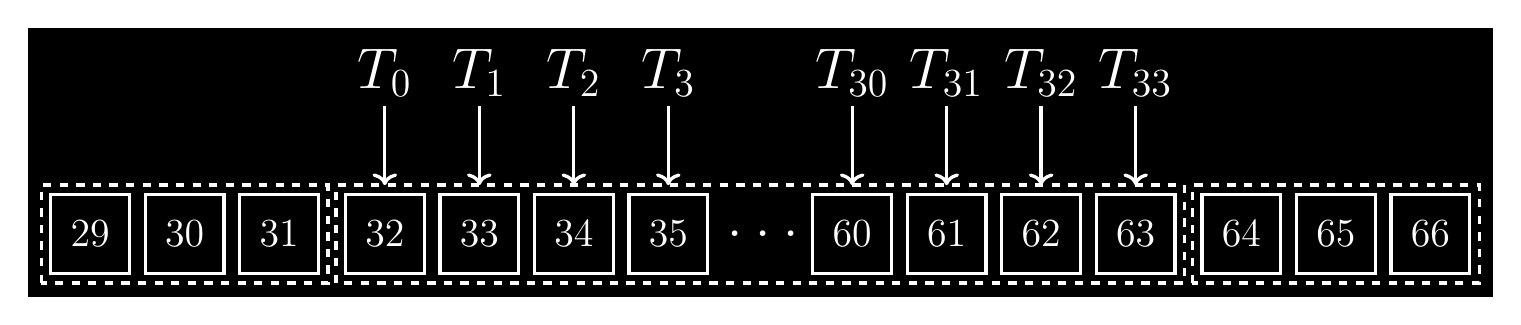
\begin{tikzpicture}[
  show background rectangle, 
  background rectangle/.style={fill=black},
  color=white,
  help lines/.style={color=lightgray,line width=.2pt},
  ]

  

  \foreach \t in {0,...,3}
   {
     \tikzmath{
       integer \x;
       \x = \t+32;
     }
     %memory
     \node (mem_\t) [rectangle,draw=white,very thick,minimum width=1.cm,minimum height=1.cm,font=\Large] at($(0,0)+(1.2*\t,0)$) {$\x$};
     
     %access
     \draw[->,very thick] ($(mem_\t.north) + (0,1.1)$) -- ($(mem_\t.north) + (0,.1)$);

     %label
     \node (label_\t) [draw=none,font=\huge,above] at($(mem_\t.north) + (0,1.1)$) {$T_{\t}$};
   }

   \node (dots_between) [font=\Huge,anchor=west] at($(mem_3.east) + (0.1,0)$) {\dots};

   \foreach \t in {0,...,3}
   {
     \tikzmath{
       integer \x, \id;
       \x = \t+30;
       \id = \t+60;
     }
     % memory
     \node (mem_\x) [rectangle,draw=white,very thick,minimum width=1.cm,minimum height=1.cm,font=\Large] at($(dots_between.east)+(.4,0)+(1.2*\t,0)$) {$\id$};
     
     %access
     \draw[->,very thick] ($(mem_\x.north) + (0,1.1)$) -- ($(mem_\x.north) + (0,.1)$);

     %label
     \node (label_\x) [draw=none,font=\huge,above] at($(mem_\x.north) + (0,1.1)$)  {$T_{\x}$};
   }
   \draw[dashed,very thick] ($(mem_0.south west) + (-.1,-.1)$) rectangle ($(mem_33.north east) + (0.1,.1)$);
   

   %right cache line
   \foreach \t in {0,...,2}
   {
     %memory
     \tikzmath{
         integer \id;
         \id = 64+\t;
       }
     \node (rcl_\t) [rectangle,draw=white,very thick,minimum width=1.cm,minimum height=1.cm,anchor=west,font=\Large] at($(mem_33.east)+(.3,0)+(1.2*\t,0)$) {$\id$};
   }
   \draw[dashed,very thick] ($(rcl_0.south west) + (-.1,-.1)$) rectangle ($(rcl_2.north east) + (0.1,.1)$);

   %left cache line
   \foreach \t in {0,...,2}
   {
     \tikzmath{
       integer \id;
       \id = 31-\t;
     }
     %memory
     \node (lcl_\t) [rectangle,draw=white,very thick,minimum width=1.cm,minimum height=1.cm,anchor=east,font=\Large] at($(mem_0.west)+(-.3,0)+(-1.2*\t,0)$) {$\id$};
   }
   \draw[dashed,very thick,draw=white] ($(lcl_2.south west) + (-.1,-.1)$) rectangle ($(lcl_0.north east) + (.1,.1)$);

\end{tikzpicture}
\end{document}
